\subsection{Free Energy Calculations}

As it is mentioned in Section \ref{subsec:TI}, The free energy difference ($\Delta G$) between two states A and B, can be calculated using Equation \ref{eq:TI}. This equation includes all the potential interactions present in the system. In this case, there are two sources of energy interactions: peptide-peptide (P-P), peptide-solvent (P-S) and solvent-solvent (S-S) interactions. (Notice that the coulomb interactions does not contribute to the Hamiltonian because each atom's charge present in the peptide, were set to 0). 
\begin{equation}
    \left \langle \frac{\partial H}{\partial\lambda} \right \rangle^{vdw}_{\lambda} = \left \langle \frac{\partial H}{\partial\lambda} \right \rangle^{vdw}_{P-P} + \left \langle \frac{\partial H}{\partial\lambda} \right \rangle^{vdw}_{P-S}.
    \label{eq:dHdl_pp}
\end{equation}
Both terms in Equation \ref{eq:dHdl_pp} contributes to the total numerical result of the free energy change between the states A and B, but, the main objective of this work is to calculate only the \textbf{free energy of forming the dry cavity} generated by the non-polar interaction ($\Delta G^{vdw}$) of the solvated solute. Taking this into account, the therm $\left \langle \frac{\partial H}{\partial\lambda} \right \rangle^{vdw}_{P-P}$ does not contribute to generate the cavity because only consider the interaction between it self, so it must be unchanged during the $\lambda$-transition, i.e, the van der Waals \textbf{peptide-peptide} interactions must remain unchanged during the process. 
This was obtain by adding an extra block (\texttt{LAMBDAS}) to the molecular dynamics input file (\textbf{*.imd}) which control the interaction between the coupling parameter $\lambda$, and the groups previously define (Sec. \ref{subsubsec:sim_box}). This allows to determine that the parameter only affects the peptide-solvent interaction, groups (1-2). Figure \ref{fig:StateAB} represent this phenomenon. 

\begin{figure}[h]
    \centering
    \begin{subfigure}[t]{0.45\textwidth}
    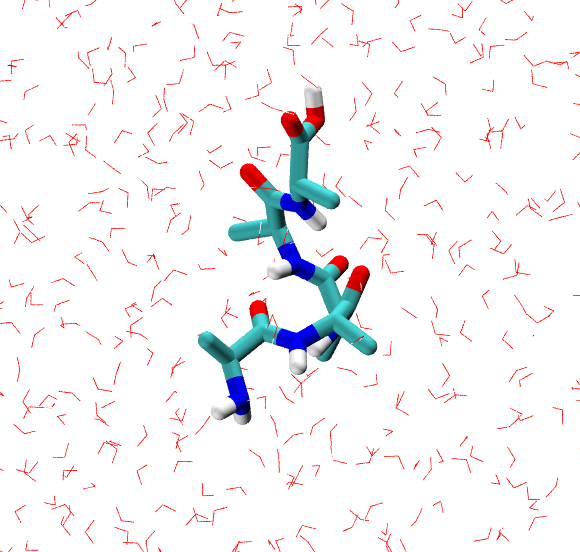
\includegraphics[width=\textwidth]{Figures/Chapter_5/StateA.png}
    \caption{Representation of state \textbf{A}. All van der Waals interactions on.}
    \label{fig:StateA}
    \end{subfigure}
    \hspace{0.5cm}
    \begin{subfigure}[t]{0.45\textwidth}
    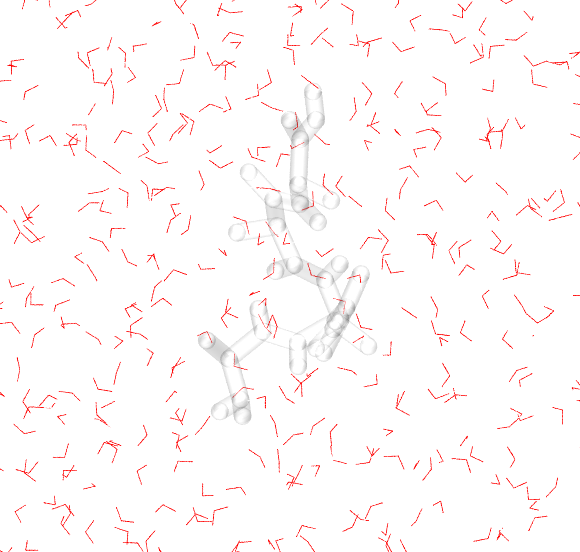
\includegraphics[width=\textwidth]{Figures/Chapter_5/StateB.png}
    \caption{Representation of state \textbf{B} with all van der Waals interactions equal to 0: the ``dummy molecule".}
    \label{fig:StateB}
    \end{subfigure}
    \caption{Graphic representation of the process of \textbf{Thermodynamic Integration} where a molecules is turn into a dummy molecule according to the couple parameter $\lambda$. The transition goes froms State A to State B.}
    \label{fig:StateAB}
\end{figure}

\subsubsection{Thermodynamic Integration's Numerical Error}\label{subsubsec:TIerror1}
To compute the free energy between state A and B, the integrate curve over all $\lambda$-steps must be calculated. For each value of $\lambda$, every $\frac{\partial H}{\partial \lambda}$ in the soft-core potential form (Sec. \ref{subsubsec:softcore}) is computed. To avoid numerical errors related to the smoothness of the curve generated, and further numerical integration, the transition over the $\lambda$-points must assure that the function generated by Equation \ref{eq:TI} is smooth enough to prevent this.
This is accomplish by simulate more $\lambda$-points in between other to generate more $\frac{\partial H}{\partial \lambda}_i$ values for the curve. In this case, five versions of TI were preformed to determine the total number of $\lambda$-steps: $[10,17,20,23,32]$. Al five versions are attached to this work in \ref{subsec:TI_evolve}. As a result of that, the $\lambda$ space, between 0 and 1 were distribute in 32 discrete points: 

\begin{table}[th] %th for exact position.
    \centering
    \begin{tabular}{|c|c|c|c|c|c|c|c|}
    \toprule
         0.000 & 0.400 & 0.600 & 0.690 & 0.715 & 0.735 & 0.800 & 0.880 \\
         0.100 & 0.450 & 0.625 & 0.700 & 0.720 & 0.740 & 0.820 & 0.900 \\
         0.200 & 0.500 & 0.650 & 0.705 & 0.725 & 0.760 & 0.840 & 0.950 \\
         0.300 & 0.550 & 0.675 & 0.710 & 0.730 & 0.780 & 0.860 & 1.000 \\
    \bottomrule
    \end{tabular}
    \caption{Distribution of 32 $\lambda$ points between 0 and 1.}
    \label{table:l_points}
\end{table}

For each window, 0.2 $[ns]$ of equilibration was performed, followed by 15 $[ns]$ of production MD, from which the free energy differences between adjacent $\lambda$ values were computed with the methods outlined above, and the total free energies were calculated by integrate the curve over all the $\lambda$-steps. 

 